Neste Capítulo serão apresentados os conceitos e principais aspectos relacionados à \textit{Workflows}, \textit{Workflows} científicos e como os chamados Sistemas Gerenciadores de \textit{Workflows} Científicos ajudam cientistas na construção destes fluxos de trabalho e no gerenciamento de seu ciclo de vida. Também apresenta alguns Sistemas de \textit{Workflows}, mostrando suas características, assim como suas vantagens e desvantagens. Para isso, a Seção \ref{cap3sec1} mostra os conceitos básico de um \textit{Workflow} Científico, a Seção \ref{cap3sec2} apresenta o seu ciclo de vida, mostrando suas fases e principais características. A Seção \ref{cap3sec3} introduz os conceitos e definições de um Sistema Gerenciador de \textit{Workflows} Científicos e na Seção \ref{cap3sec4} são apresentados alguns exemplos desses sistemas, consolidados nos meios acadêmicos e comercial. Por fim, na Seção \ref{cap3sec5} são descritas as vantagens percebidas ao se utilizar um Sistema Gerenciador de \textit{Workflows} Científicos.

\section{Conceitos e Definições} \label{cap3sec1}

Um \textit{workflow} é uma sequência de passos bem definidos usados para automatizar algum processo, de acordo com um conjunto de regras definidas, permitindo que estes possam ser executados por uma outra pessoa gerando a mesma saída. Nessa automação, documentos, informações ou tarefas são processados, de acordo com um conjunto de procedimentos. Um \textit{workflow} é composto de grupos de dados, fases de análise, fluxos e ferramentas ordenados de maneira a se atingir o objetivo desejado. Nesse contexto, existem diversos software computacionais, que utilizam uma gama enorme de tecnologias diferentes, que possuem a tarefa de gerenciar o ciclo de vida de um \textit{workflow}. Esses sistemas são geralmente conhecidos como Sistemas Gerenciadores de \textit{Workflow} (\textit{WfMS - Workflow Management Systems}), e garantem que os passos que automatizam os processos ocorrem na sequência correta.

No contexto da Bioinformática, as análises computacionais dos dados obtidos por meio de sequenciadores automáticos são realizadas em diferentes fases, ou passos. Para cada fase, existe um conjunto de ferramentas de Bioinformática a ser utilizado. Entretanto, cada tipo de pesquisa implica numa combinação diferente de ferramentas, de acordo com os objetivos da pesquisa, e este fluxo de passos é chamado de \textit{workflow} de Bioinformática. Esse dinamismo gera uma complexidade adicional ao projeto, pois é necessário implementar mecanismos de gerenciamento dessa entidade (\textit{workflow}) a cada nova pesquisa, assim como os dados utilizados em suas entradas (\textit{inputs}) e saídas (\textit{outputs}).

De acordo com Singh \textit{et al.} [21][22] um \textit{workflow} científico é definido como ``\textit{uma série de atividades estruturadas e cálculos que surgem na resolução de problemas científicos}'', e um ``\textit{processo automatizado que combina dados e processos em um conjunto estruturado de passos para implementar soluções computacionais para um problema científico}''. \textit{Workflows} científicos distinguem-se de \textit{workflows} de negócio (\textit{business workflows}) pois contém fluxos centrados nos dados [23][24], são mais flexíveis [25] e são utilizados principalmente para descrever a execução de experimentos científicos [25].

Um dos objetivos de se utilizar \textit{workflows} científicos é apoiar e, sempre que possível, automatizar fases como visualização, tarefas repetitivas, o acesso aos dados, transformação, análise e que, se feitas de outra maneira, estariam propensas a erros. Assim, \textit{workflows} científicos são muitas vezes usados para encadear aplicativos especializados e de novos métodos de análise de dados. No entanto, assim como ocorre em \textit{workflows} de negócios, \textit{workflows} científicos não são apenas mecanismos de gerenciamento da execução de uma sequência de passos. Outras áreas como modelagem, \textit{design}, análise e reutilização de \textit{workflows} estão se tornando cada vez mais importante neste contexto. Assim, as principais vantagens ao se utilizar \textit{workflows} científicos são: \textit{(i)} auxiliar pesquisadores permitindo que eles se concentrem no domínio específico do seu trabalho, ao invés de perder tempo lidando com complexas questões de gestão de dados e de software complicados; e \textit{(ii)} evitar desperdícios de poder computacional, otimizando a execução de \textit{workflow} sobre os recursos disponíveis.

A Seção seguinte trata da conceituação do ciclo de vida de um \textit{workflow}, suas etapas e principais aspectos.

\section{Ciclo de Vida de um \textit{Workflow}} \label{cap3sec2}

As várias fases e etapas associadas ao desenvolvimento, implantação e execução de \textit{workflows} científicos compreendem o seu ciclo de vida [30]. Essas fases são em grande parte suportadas por sistemas gerenciadores de workflow existentes (\textit{WfMS - Workflow Management System}), utilizando uma ampla variedade de abordagens e técnicas. A Figura \ref{fig:ciclo_vida_workflow} demonstra o ciclo de vida de um \textit{workflow}, e suas fases podem ser descritas da seguinte maneira:

\begin{figure}[H]
	\centering
	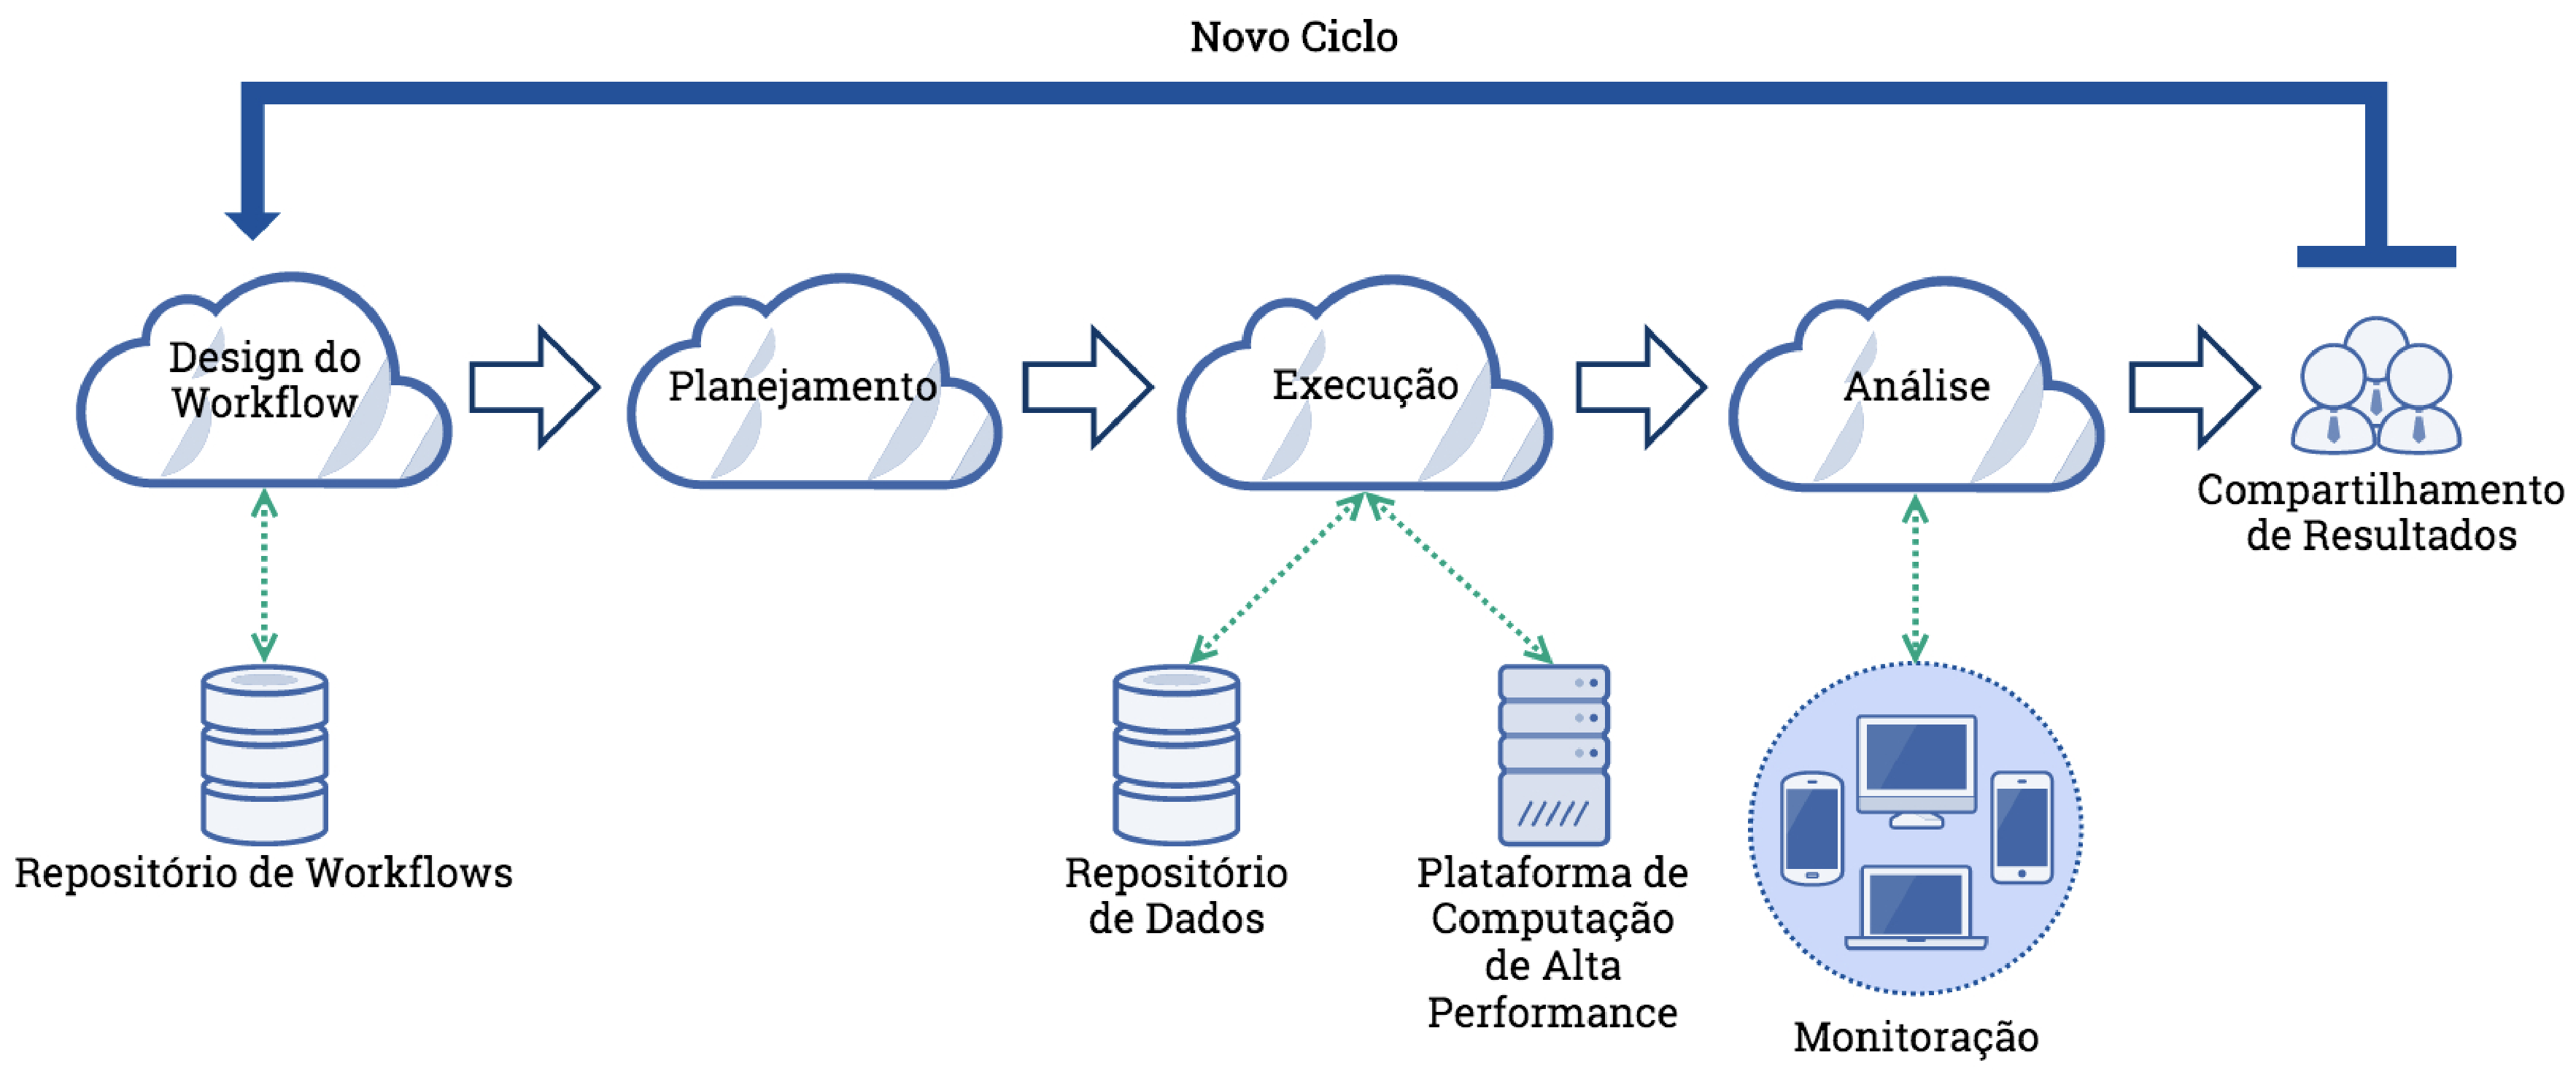
\includegraphics[scale=0.27]{ciclo_vida_workflow.pdf}
	\caption{Ciclo de Vida de um \textit{Workflow}.}
	\label{fig:ciclo_vida_workflow}
\end{figure}

\begin{itemize}
	\item \textbf{Projeto e Composição:} O desenvolvimento de \textit{workflows} científicos geralmente começa com o levantamento de requisitos dos cientistas envolvidos em uma pesquisa. Uma especificação das funcionalidades do \textit{workflow} desejado é criada, e então um \textit{workflow} é montado com base nesta especificação. O desenvolvimento de um \textit{workflow} difere da programação tradicional de muitas maneiras. Normalmente, seu desenvolvimento abrange a composição e a configuração de um \textit{workflow} para fins especiais de componentes, \textit{subworkflow} e serviços pré-existentes. A construção de \textit{workflows} assemelha-se mais à programação \textit{Script} do que o desenvolvimento de aplicações convencional. Durante a composição do \textit{workflow}, o usuário ou cria um novo \textit{workflow} modificando um existente, ou então compõe um novo \textit{workflow} a partir do zero usando componentes e \textit{subworkflows} obtidos a partir de um repositório externo. Em contraste com o conceito de \textit{workflows} de negócios, onde padrões foram desenvolvidos ao longo dos anos (por exemplo, mais recentemente WS-BPEL 2.0 [JE07]), sistemas de \textit{workflow} científicos tendem a usar a sua própria linguagem e formatos de troca (por exemplo, SCUFL [Tav], GPEL [WHH05], e MOML [BLL + 08], entre outros). As razões para esta divergência são a vasta gama de modelos de computação (Computação em Nuvem, por exemplo) utilizados na construção de \textit{workflows} científicos e o foco do desenvolvimento das funcionalidades envolvidas, que no caso são orientadas para o cientista.
    \item \textbf{Planejamento de Recursos:} Assim que a descrição do \textit{workflow} é construída, sistemas gerenciadores de \textit{workflows} científicos muitas vezes fornecem várias funcionalidades antes da execução. Essas funções podem incluir a validação (por exemplo, verificação de tipo), a alocação de recursos, a programação, a otimização, os parâmetros de execução e a escolha de dados de entrada. Mapeamento de \textit{workflows} é por vezes utilizado para se referir às decisões de otimização e programação feitas durante a fase de planejamento de recursos. Em particular, durante a fase de concepção e composição, os recursos de destino a serem utilizados para a execução não são tipicamente escolhidos. Mapeamento de fluxo de trabalho, então, refere-se ao processo de geração de um \textit{workflow} executável baseada em uma descrição abstrata do \textit{workflow} independente de recurso [DBG + 03]. Em alguns casos, o usuário executa o mapeamento diretamente escolhendo os recursos adequados. Em outros casos, o sistema gerenciador do \textit{workflow} executa automaticamente o mapeamento. Neste último caso, os usuários tem permissão para construir \textit{workflow} em um nível de abstração acima, não definindo aspectos do ambiente de execução.
    \item \textbf{Execução:} Uma vez que um \textit{workflow} é mapeado e dados foram selecionados e colocados à disposição do sistema gerenciador de \textit{workflows}, o mesmo pode ser executado. Durante a execução, um sistema gerenciador de \textit{workflows} pode registrar o histórico dos processos, bem como fornecer funções de monitoramento e \textit{failover} (recuperação em caso de falha) em tempo real. Dependendo do sistema, geralmente é realizada a gravação dos passos que foram invocadas durante a execução do \textit{workflow}, os dados consumidos e produzidos por cada passo, um conjunto de dependências, e assim por diante. Um \textit{workflow} pode mudar durante sua execução (por exemplo, devido a mudanças na disponibilidade de recursos), assim, a evolução deste \textit{workflow} é dinâmica e deve ser registrada, a fim de dar suporte a análise posterior de sua execução.
    \item \textbf{Análise da Execução:} Após a execução do \textit{workflow}, os cientistas envolvidos muitas vezes precisam inspecionar e interpretar os resultados gerados pelo \textit{workflow}. Isso envolve a avaliação daquilo que foi produzido (ou seja, se o resultado faz sentido), examinar os rastros de execução do \textit{workflow} (verificar o passo a passo da execução até se chegar ao resultado), depurar o \textit{workflow} (verificar possíveis erros), e análise de desempenho (examinar o tempo gasto por cada passo).
    \item \textbf{Compartilhamento dos Resultados:} Dados e o produto do \textit{workflow} podem ser publicados e compartilhados entre o grupo de pessoas envolvidas. A partir do momento em que os dados gerados pela execução do \textit{workflow} são enviados para um repositório compartilhado, novas iterações do ciclo de vida do \textit{workflow} podem começar novamente.
\end{itemize}    
    
Outro aspecto muito importante na manutenção de \textit{workflows} científicos é definir os papéis dos usuários do sistema (\textit{User Roles}) [30]. Cada usuário possui uma função específica e bem definida no controle do ciclo de vida de um \textit{workflow}. Dessa forma, os usuários de sistemas gerenciadores de \textit{workflows} científicos podem desempenhar uma série de funções diferentes dentro das fases indicadas. Um \textit{designer} de \textit{workflows} é geralmente um cientista que desenvolve um novo protocolo experimental ou analítico (ou uma nova variante de um método existente). 

Como mencionado, um projeto de \textit{workflow} é muitas vezes provocado por alguma forma de análise de requisitos. Assim, o desenho e os requisitos associados podem ser usados por um engenheiro de \textit{workflows} para a implementação da descrição abstrata ou executável do \textit{workflow} associado. Um operador do \textit{workflow} é um usuário que executa \textit{workflows} utilizando as entradas desejadas. Um operador pode iniciar um \textit{workflow} diretamente através de um sistema gerenciador de \textit{workflows} científicos, ou indiretamente através de outro aplicativo (por exemplo, dentro de um portal web), monitorar a sua execução (por exemplo, através de um \textit{dashboard}) e, posteriormente, validar os resultados obtidos. Os papéis de usuário acima descritos não são necessariamente disjuntos. Por exemplo, uma única pessoa pode assumir os papéis de \textit{designer}, de engenheiro e de operador do \textit{workflow}. 

Dessa forma, sistemas gerenciadores de \textit{workflows} científicos visam tornar o projeto, a execução e o resultado da análise mais fácil em comparação com abordagens baseadas em \textit{script} tradicionais para automação de processos científicos.

Na Seção \ref{cap3sec3} serão abordados características dos chamados sistemas gerenciadores de \textit{workflows} científicio

\section{Sistemas Gerenciadores de \textit{Workflows} Científicos} \label{cap3sec3}

A tecnologia da informação está revolucionando a forma que muitas pesquisas são conduzidas, com novas técnicas e modelos de computação, em campos multidisciplinares, tais como Bioinformática, Informática Biomédica, Quimioinformática, Geoinformática, etc. Para avançar ainda mais nessa nova ciência orientada a dados e à informação através da utilização de avançada infraestrutura de TI, grandes investimentos são realizados. Enquanto muitos esforços se concentram no desenvolvimento dessa infraestrutura, com novas tecnologias de \textit{grid} e, mais recentemente, a utilização de nuvens computacionais, cientistas estão interessados em ferramentas, como bancos de dados distribuídos e recursos de \textit{grids} computacionais, que permitam-lhes projetar, montar e executar seus próprios \textit{workflows} científicos. 

Idealmente, o cientista deve ser capaz de ligar qualquer recurso de dados científicos e serviços computacionais em um \textit{workflow} científico, inspecionar e visualizar dados à medida que são processados, fazer alterações de parâmetros quando necessário executar novamente apenas os componentes afetados por um possível erro. Assim, um sistema de \textit{workflows} científicos torna-se um ambiente de resolução de problemas científicos, sintonizado cada vez mais com a utilização de infraestruturas de sistemas distribuídos como \textit{grids} e nuvens computacionais.

\section{Exemplos de Sistemas Gerenciadores de \textit{Workflows} Científicos} \label{cap3sec4}

Nesse cenário de utilização de infraestrutura de TI para otimizar o projeto, a execução e a análise de \textit{workflows} científicos, diversas propostas de sistemas surgiram utilizando uma vasta gama de técnicas, infraestruturas e tecnologias, tais como: DiscoveryNet [34], Taverna [35], Triana [36], Kepler [37] e Pegasus [38][39]. No que diz respeito a esses sistemas gerenciadores, seguem abaixo algumas características e aspectos principais. \\

% Scientific Workflow Systems 

\noindent
\textbf{\textit{DiscoveryNet}} \\

\noindent
O sistema \textit{Discovery Net} foi concebido em torno de um modelo de \textit{workflows} científicos para a integração de fontes de dados distribuídos e ferramentas analíticas dentro de uma infraestrutura de \textit{Grid}. O sistema foi originalmente desenvolvido como parte do projeto financiado de \textit{e-Science} do Reino Unido, \textit{Discovery Net} (2001-2005) com o objetivo de produzir uma plataforma orientada para aplicações de alto nível, com foco na capacitação de cientistas na derivação de novos conhecimentos a partir de dispositivos, sensores, bancos de dados, componentes de análise e recursos computacionais acessíveis pela Internet. Seu conjunto dedicado de componentes para a mineração de dados tem sido usado como base para inúmeros projetos de diversos domínios do conhecimento. Muitas das ideias de pesquisa desenvolvidas no âmbito do \textit{Discovery Net} também foram incorporadas dentro do sistema IDBS (antigo InforSense KDE) [44], um sistema de mineração de dados e \textit{workflows} de gerenciamento comercial que tem sido amplamente utilizada para aplicações de negócios orientados. 
    
\begin{figure}[ht]
	\centering
	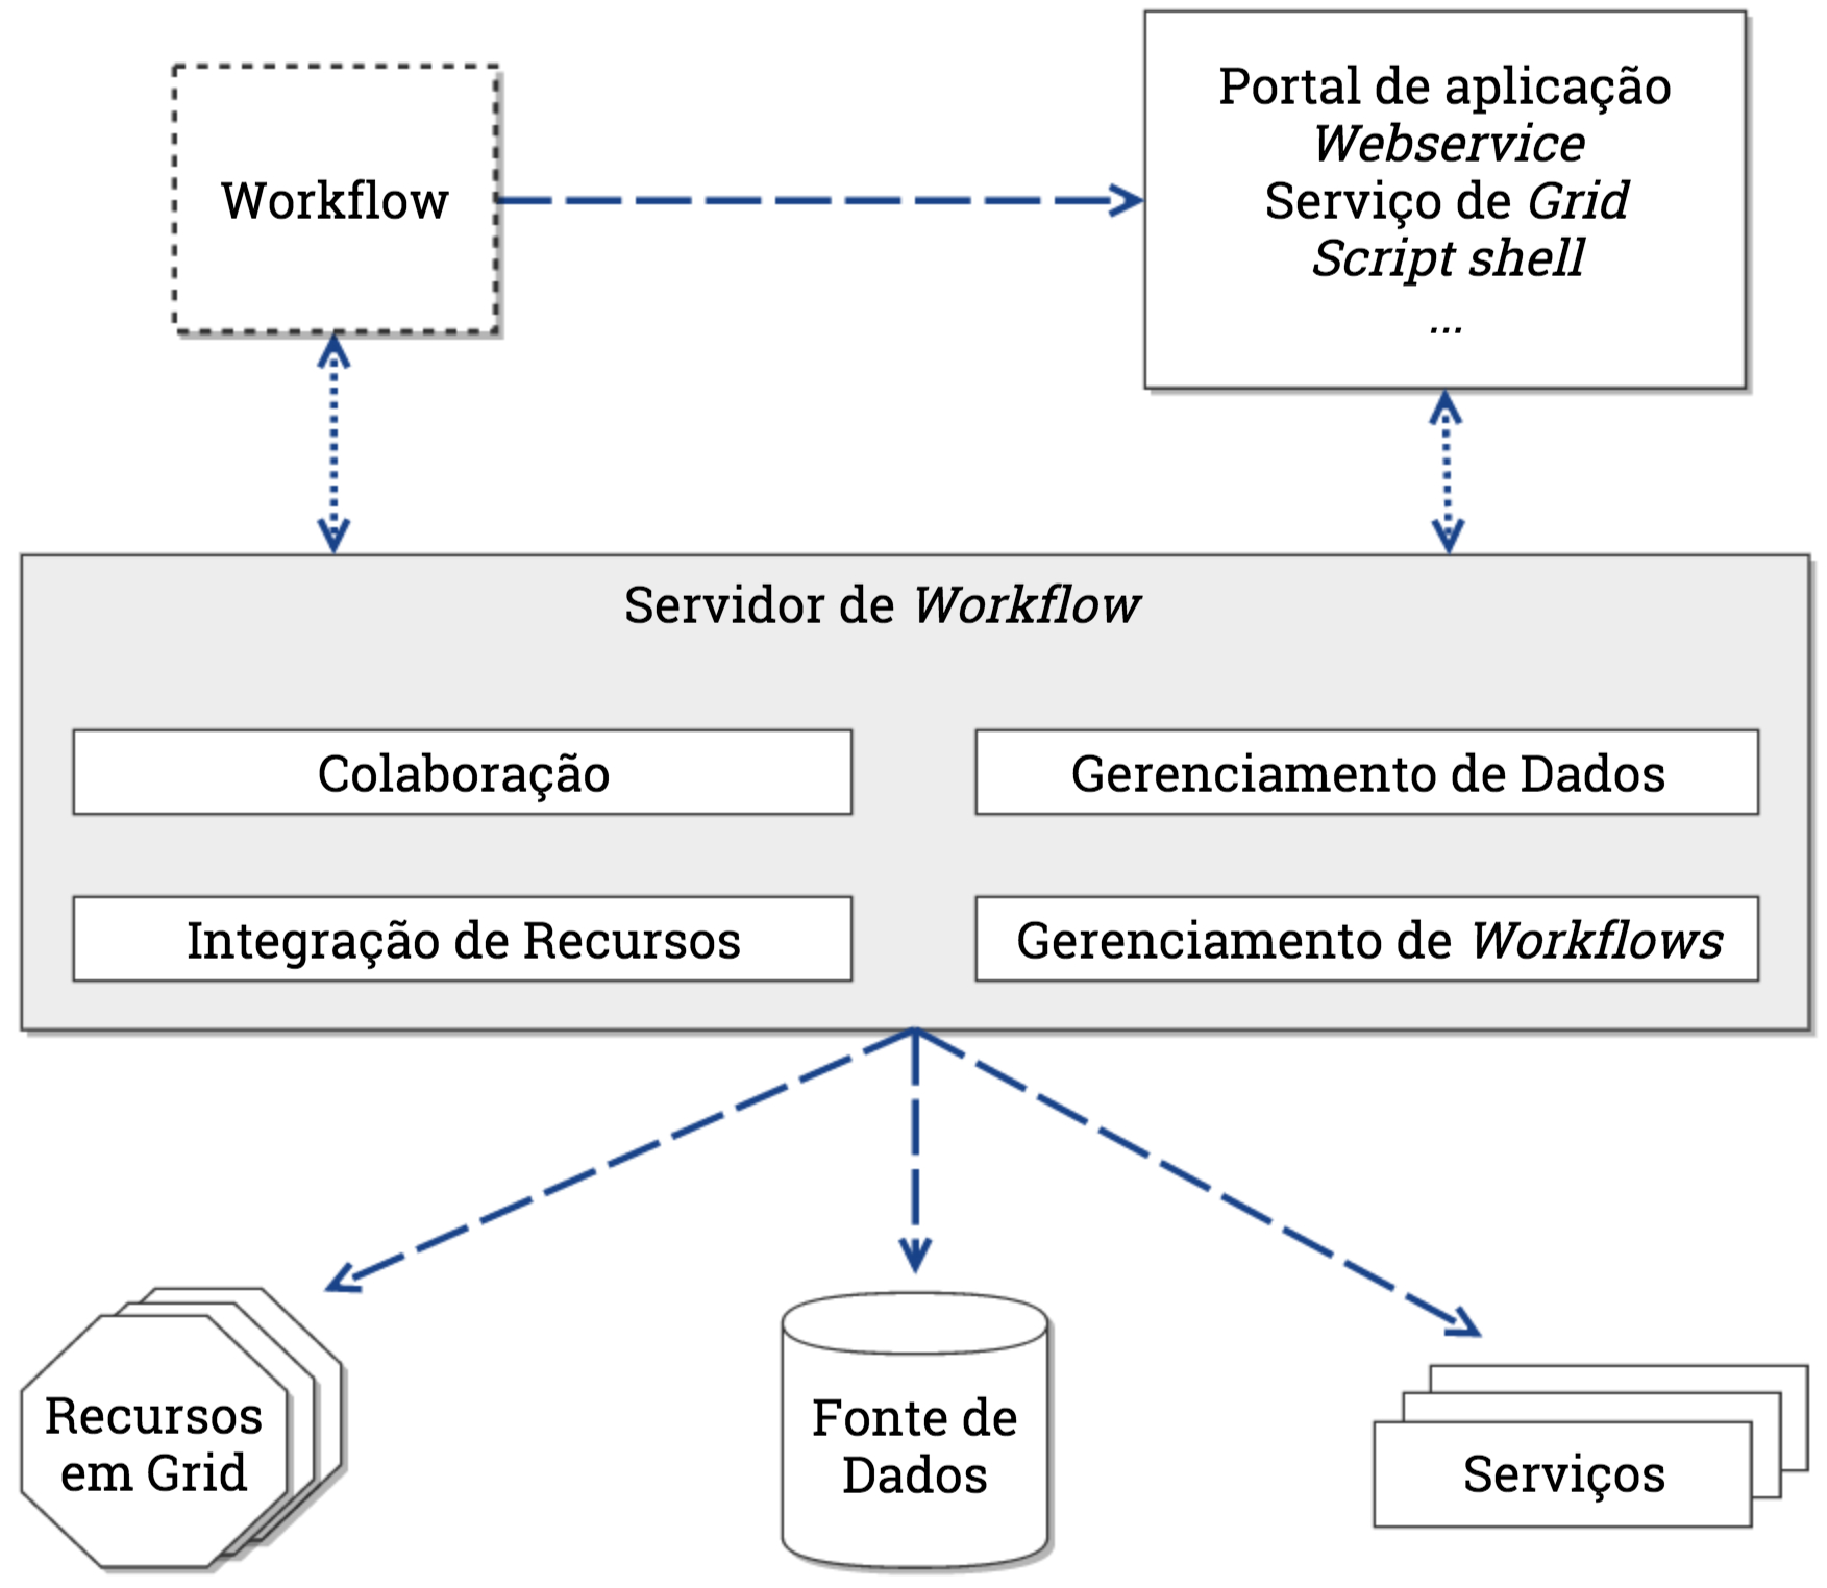
\includegraphics[scale=0.43]{arquitetura_discoverynet.pdf}
	\caption{Arquitetura multicamada do \textit{DiscoveryNet} (adaptado de \cite{can_one_size_fit_all}).}
	\label{fig:arquitetura_discoverynet}
\end{figure}  
    
A Figura \ref{fig:arquitetura_discoverynet} fornece uma visão geral de alto nível do \textit{Discovery Net}. O sistema é baseado em uma arquitetura multicamada, com um servidor de \textit{workflows}, fornecendo funções necessárias para a criação e execução de \textit{workflows}, tais como a integração e acesso a dados e recursos computacionais remotos, ferramentas de colaboração, publicação e mecanismos de visualização. O projeto do sistema tem como alvo os especialistas do domínio, ou seja, cientistas, ao invés do foco em desenvolvedores de sistemas distribuídos. Os \textit{workflows} criados desta forma também podem ser executado a partir de interfaces especializadas baseadas em tecnologias \textit{web}. A implementação do sistema em si tem evoluído ao longo dos últimos anos, a partir de um protótipo direcionados a projetos específicos de um sistema de força industrial amplamente utilizado por organizações comerciais e acadêmicas. \\

\noindent
\textbf{\textit{Taverna}} \\

\noindent
O principal objetivo do Taverna é satisfazer as necessidades dos cientistas de bioinformática que precisam construir \textit{workflows} científicos a partir de inúmeros \textit{webservices} disponíveis remotamente através da Internet. Dessa forma, existe um esforço significativo no desenvolvimento do sistema Taverna para a aquisição e organização desses \textit{webservices} em uma coleção útil de componentes. Seus principais requisitos são:
    
    \begin{enumerate}
		\item 
	\end{enumerate}

Taverna foi construído utilizando-se o \textsuperscript{my}Grid [], que é um projeto de construção de \textit{middleware} que suporta o desenvolvimento de \textit{workflows} baseados em experimentos \textit{in silico} (experimentos realizados através de simulações computacionais) de Biologia. Financiado pelo Programa \textit{e-Science} do Reino Unido a partir de 2001, \textsuperscript{my}Grid tem desenvolvido um conjunto de componentes de código aberto que pode ser usado de forma independente e em conjunto. Estes incluem um diretório de serviços, ferramentas de pesquisa atuantes em descrições semânticas de recursos e dados externos; repositórios de dados e metadados semanticamente dirigidos para a gravação de um \textit{workflow} e seu ciclo de vida, bem como outros componentes, tais como processamento distribuído de consultas (\textit{queries}) e notificação de eventos. Dessa forma, Taverna foi projetado para ser o ambiente de desenvolvimento e execução de \textit{workflows} baseado em componentes do projeto \textsuperscript{my}Grid.

Taverna é um nome comum usado para o sistema de \textit{workflows} científicos que compreende o \textit{Workbench} Taverna, que é uma ferramenta gráfica de criação de \textit{workflows}, o servidor Taverna, utilizado para execução remota de \textit{workflows}, seu conjunto de ferramentas de linha de comando (\textit{Command Line Tool}) e, mais recentemente, o Taverna \textit{Online}, que é a versão deste sistema disponível pela Internet. A Figura \ref{fig:tela_taverna} mostra a interface percebida pelo usuário ao se utilizar o Taverna em sua versão online. \\

\begin{figure}[ht]
	\centering
	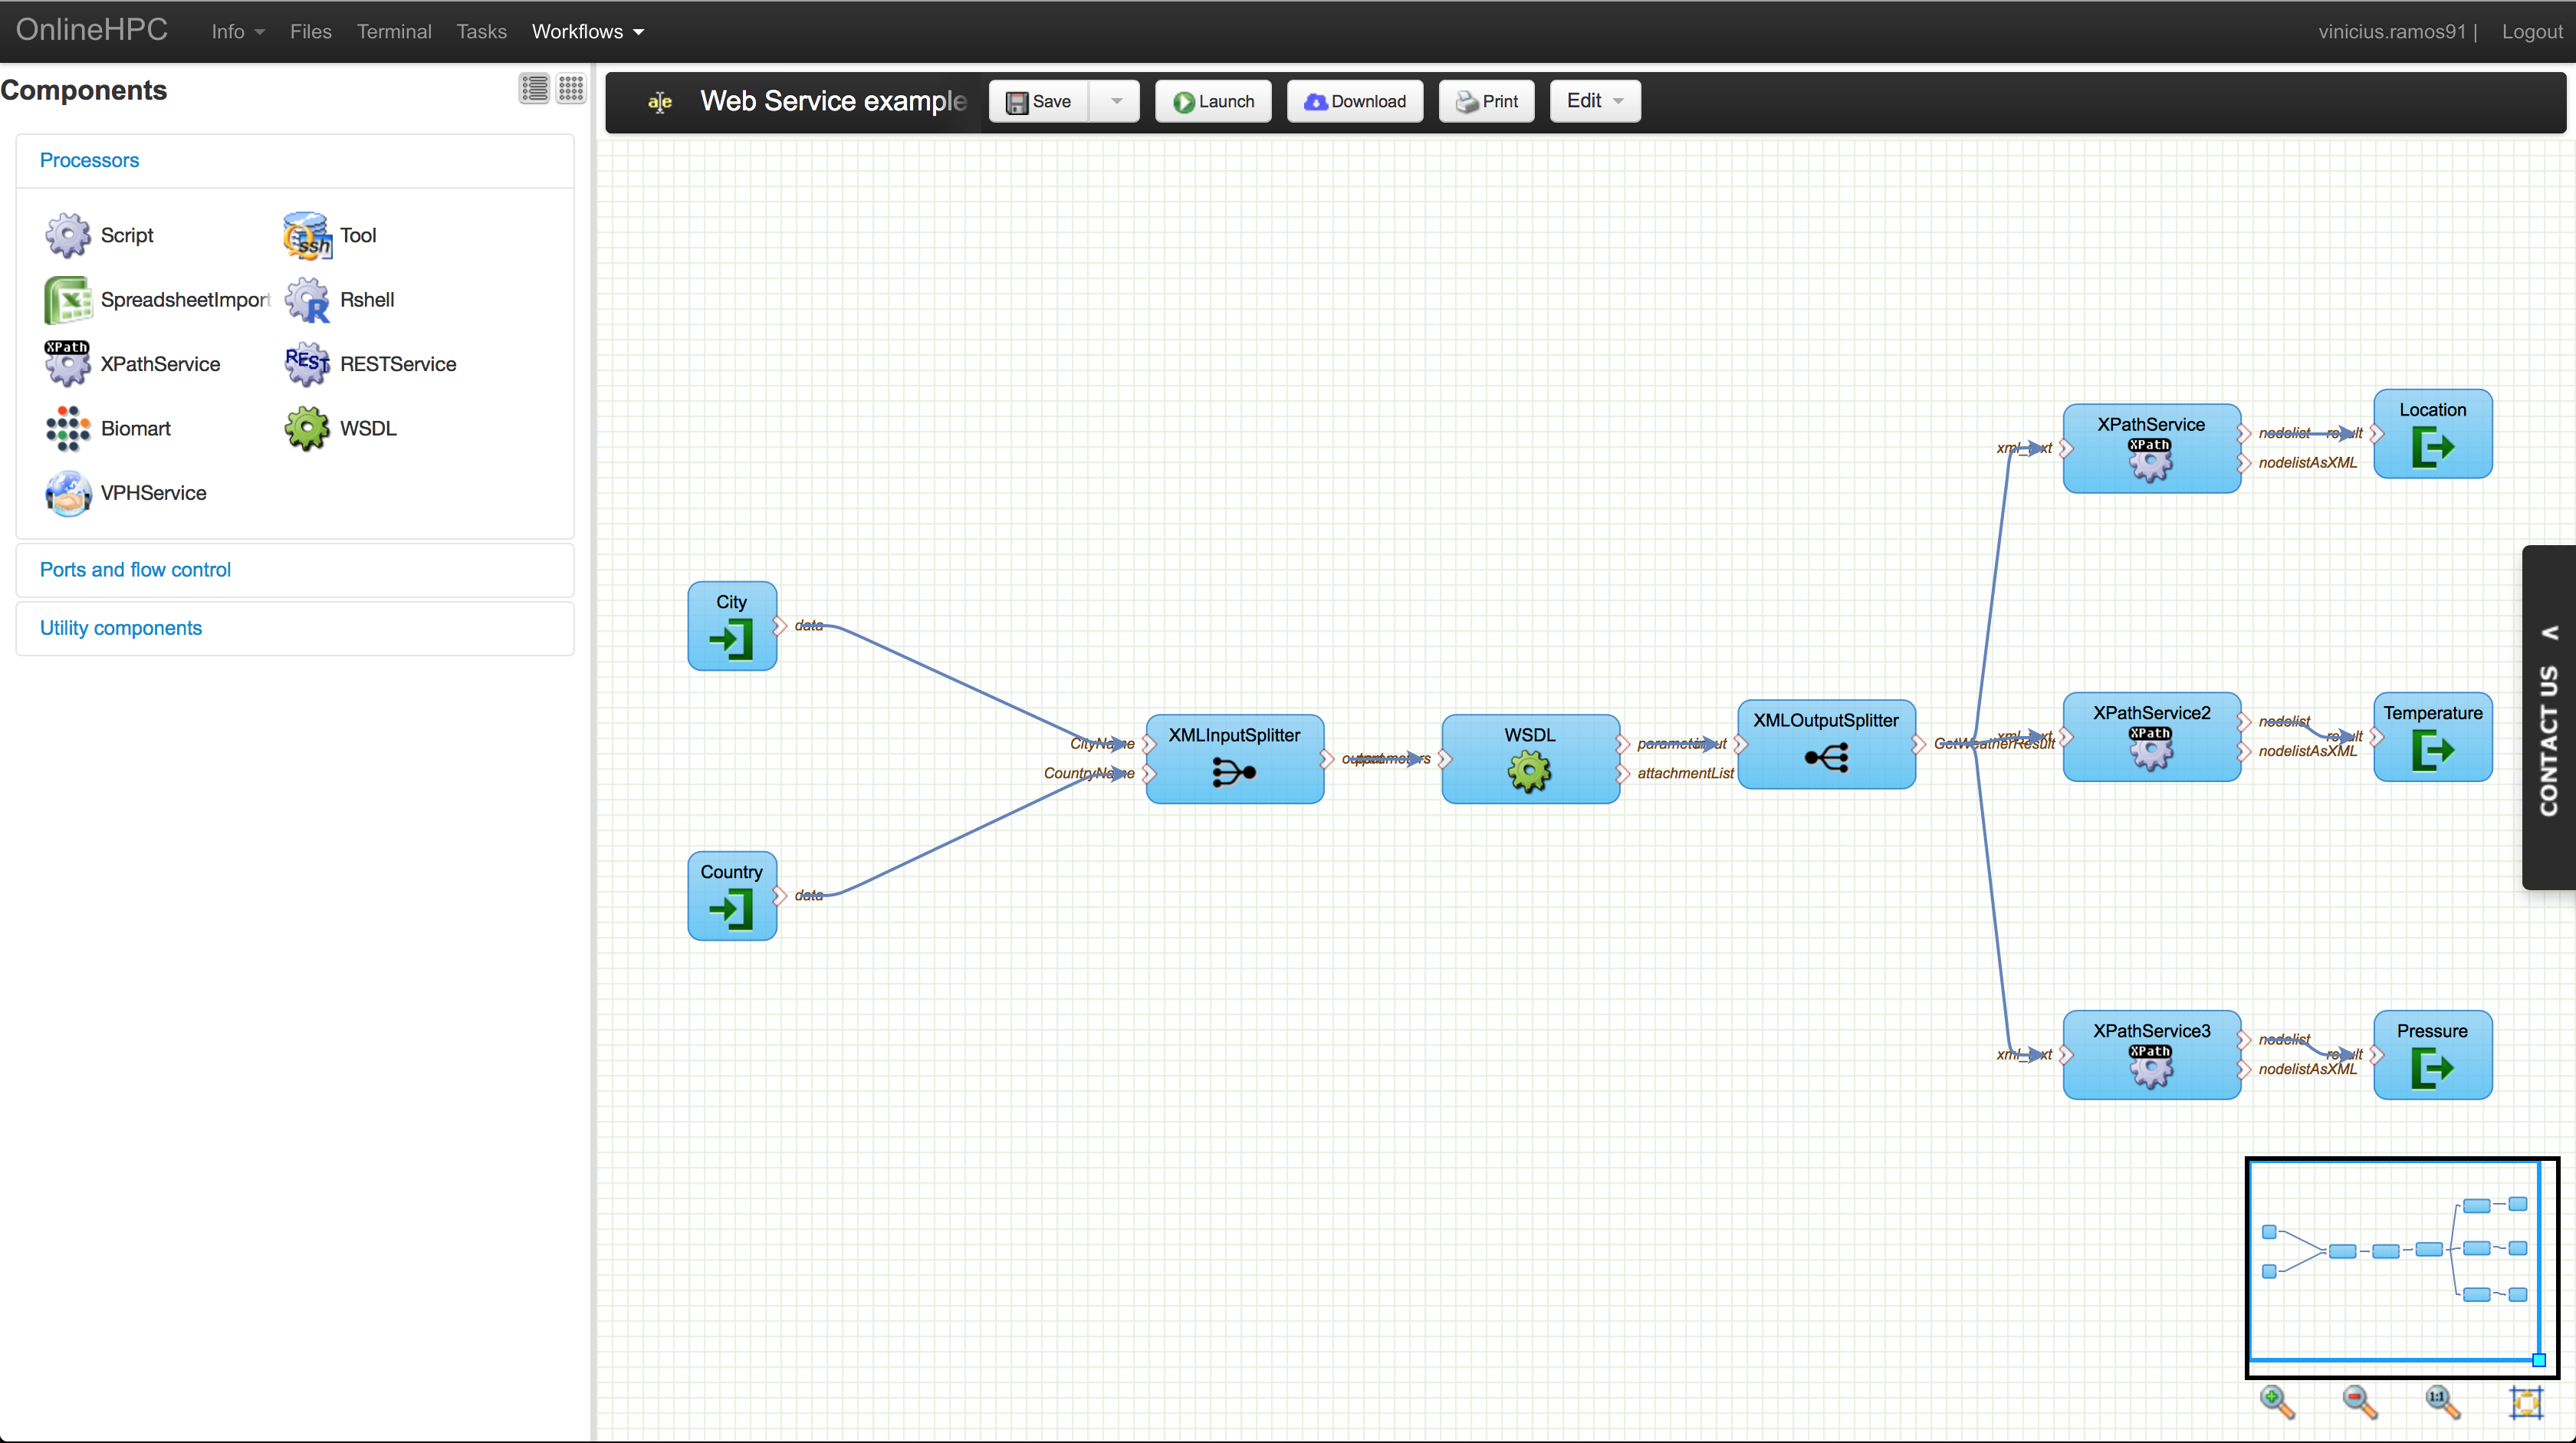
\includegraphics[scale=0.27]{tela_taverna_online.png}
	\caption{Ambiente gráfico do Taverna Online (retirado de \cite{taverna_screen}).}
	\label{fig:tela_taverna}
\end{figure}
 
\noindent
\textbf{\textit{Triana}} \\

\noindent 
Triana \cite{triana_1} \cite{can_one_size_fit_all} é uma plataforma \textit{open source}, distribuída, independente de plataforma, escrita na linguagem de programação Java utilizada como Ambiente de Resolução de Problemas (\textit{PSE - Problem Solving Environment}). Um \textit{PSE} é um ambiente de computação completo e integrado para composição, compilação e execução de aplicativos em uma área específica \cite{problem_solving}. 

O Triana é um ambiente gráfico interativo que permite aos usuários compor aplicações e especificar seu comportamento de maneira distribuída. Conforme pode ser visto na Figura \ref{fig:tela_triana}, o usuário cria um \textit{workflow} arrastando as unidades desejadas para a área de trabalho e interliga estes arrastando uma ligação entre eles. Embora o foco aqui seja a interface gráfica, Triana é composto por um conjunto complexo de componentes de interação com potencial de criar sistemas completos ou qualquer subconjunto dele. 

\begin{figure}[ht]
	\centering
	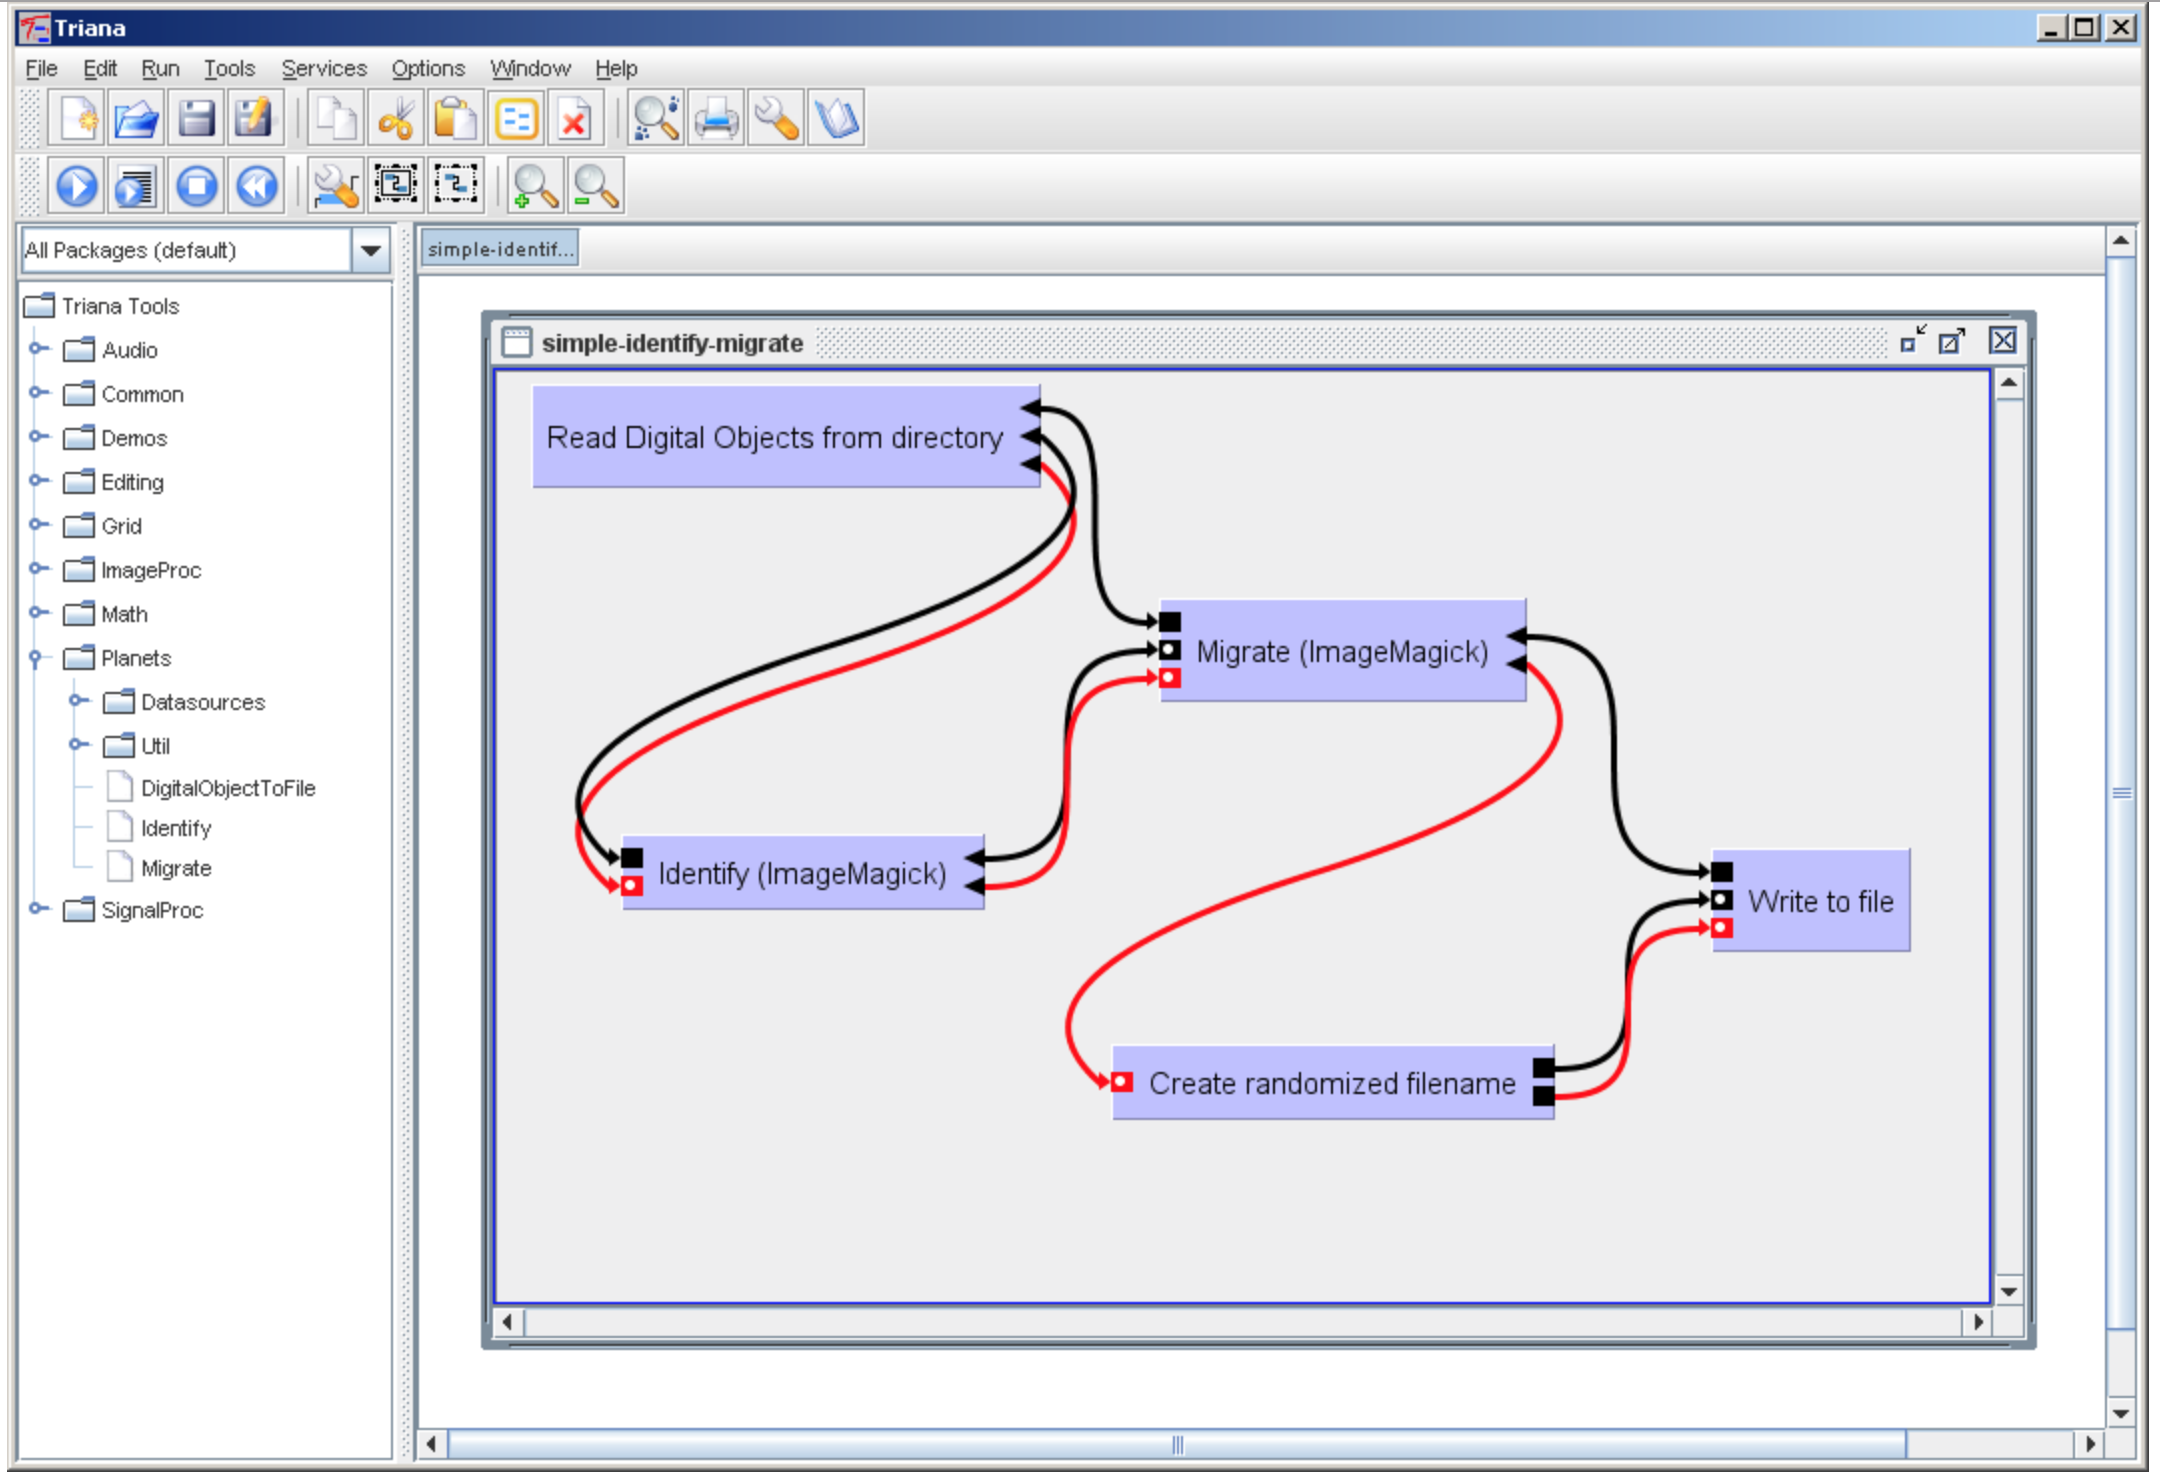
\includegraphics[scale=0.4147]{tela_triana.png}
	\caption{Ambiente gráfico do Triana (retirado de \cite{triana_screen}).}
	\label{fig:tela_triana}
\end{figure}

Esta abordagem dá ao Projeto Triana a flexibilidade necessária para ser aplicado a muitos cenários diferentes e em muitos níveis diferentes. Por exemplo, ele pode ser usado como uma base para aplicações de \textit{workflows} em \textit{grids}, para conectar componentes de \textit{grid} orientados a dados e gerenciar o \textit{workflow} entre eles, ou como um sistema de análise de dados para aplicações de imagem, processamento de sinais ou texto, permitindo que um cientista possa aplicar rapidamente algoritmos em conjuntos de dados e visualizar os resultados. 

Triana também pode ser usado como um editor gráfico de \textit{scripts} de alto nível para a criação de \textit{workflows} baseados em \textit{scripts}.\\

\noindent
\textbf{\textit{Kepler}} \\

\noindent
Kepler é um sistema para construção, composição e mecanismo de orquestração de \textit{workflows} científicos, desenvolvido a partir do Sistema \textit{Ptolemy} II \cite{ptolemy}, que é uma ferramenta de modelagem orientada ao ``ator'' (\textit{actor-oriented modeling tool}) \cite{can_one_size_fit_all}. 

O foco de Kepler é na análise de dados e modelagem de maneira genérica. Assim, Kepler é adequado para modelar processos em uma ampla variedade de domínios científicos, desde modelos físicos até \textit{webservices} de bioinformática. Ao invés de tentar fornecer uma semântica genérica para todos possíveis tipos de processos encontrados nestes domínios, Kepler separa o mecanismo de execução do \textit{workflow} e atribui um modelo de computação, chamado diretor (\textit{director}) \cite{kepler_system}, para cada \textit{workflow}. Os componentes do \textit{workflow} no Kepler são chamados de atores (\textit{actors}) e representam operações ou fontes de dados, com um determinado número de portas, podendo ser entrada, saída, ou ambos, os quais atuam como pontos finais (\textit{end-points}) para conexões. A interação entre esses componentes pode ser vista na Figura \ref{fig:actor_director}.

\begin{figure}[ht]
	\centering
	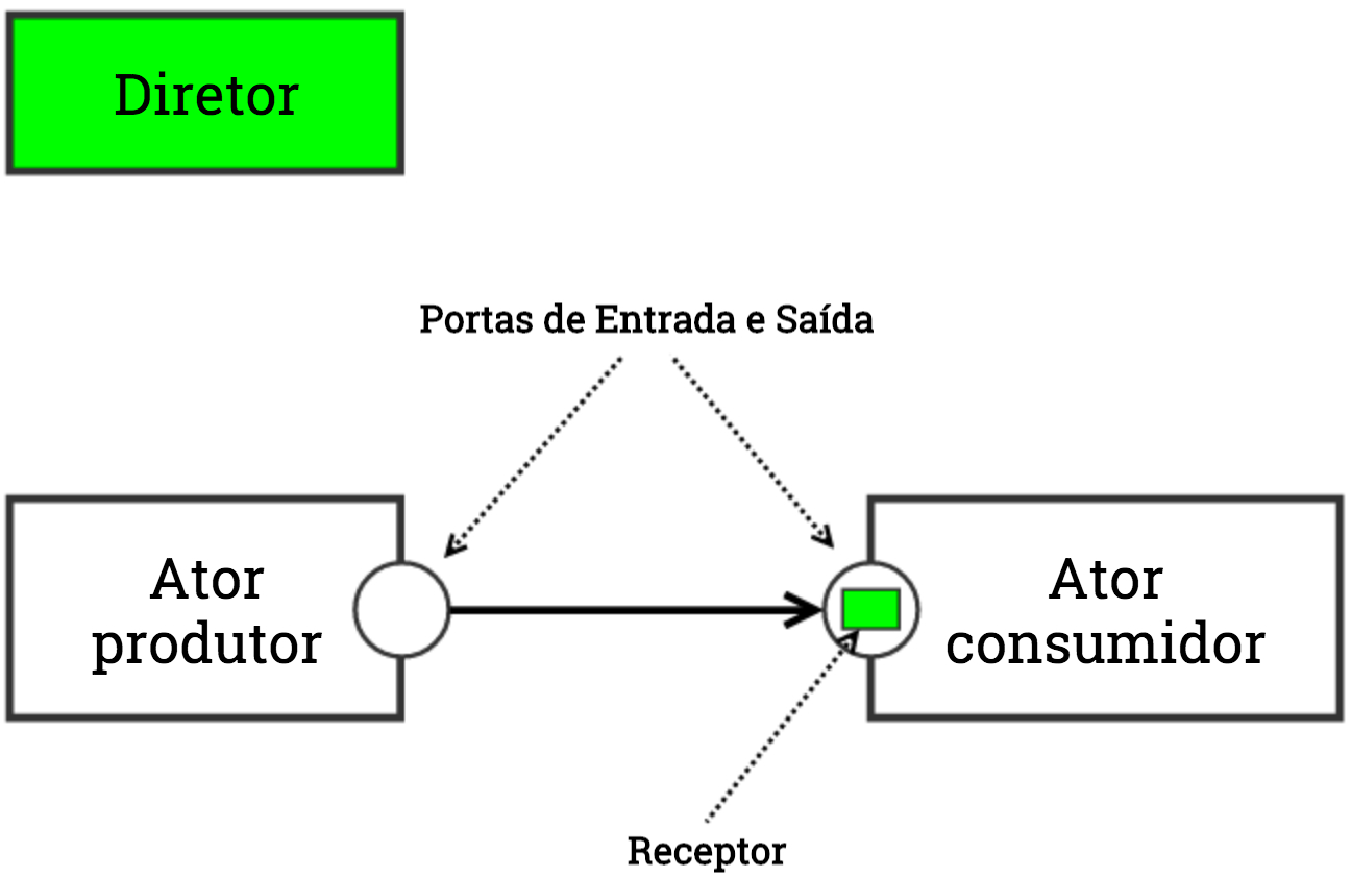
\includegraphics[scale=0.53]{actor_director.pdf}
	\caption{A semântica da interação entre os componentes é determinada pelo \textit{director}, o qual controla a execução (adaptado de \cite{kepler_system}).}
	\label{fig:actor_director}
\end{figure}

A interação mais simples consiste em um \textit{actor} consumir um conjunto de dados sobre cada porta de entrada e produzir um sinal de saída sempre que ele executa. No entanto, existem numerosos casos onde mais do que um sinal pode ser consumido (ou produzido) para cada execução.

\textit{Director} é um conceito-chave no sistema Kepler. Enquanto \textit{actors} e relações, juntos, constituem um modelo de \textit{workflow}, os \textit{directors} se encontram em um nível acima, formando seu modelo de execução ou modelo de computação (\textit{MoC - Model of Computation}). Nesta configuração, um \textit{actor} só tem conhecimento da operação a ser executada e que saídas serão produzidas. A decisão de como e quando escalonar a execução de cada \textit{actor} é deixado para o \textit{director}. Por exemplo, uma operação de adição pode aceitar dados de entrada fornecidos por diversos mecanismos, incluindo eventos discretos, envio de dados e passagem assíncrona de mensagens (\textit{asynchronous message passing}). Portanto, dependendo do \textit{director} utilizado, os \textit{actors} podem ter \textit{threads} de controle separadas, ou eles podem ter suas execuções desencadeada pela disponibilidade de uma nova entrada.

Usando Kepler, os cientistas podem capturar seus \textit{workflows} em um formato que pode ser facilmente compartilhado, arquivado, versionado, e executado. A interface gráfica intuitiva de Kepler (herdada do sistema \textit{Ptolemy}), a qual pode ser vista na Figura \ref{fig:tela_kepler}, e sua modelagem orientado à atores (\textit{actor-oriented modeling}) o tornaram uma ferramenta muito versátil para o gerenciamento do ciclo de vida de um \textit{workflow} científico para ambos engenheiros de \textit{workflows} e usuários finais.

\begin{figure}[ht]
	\centering
	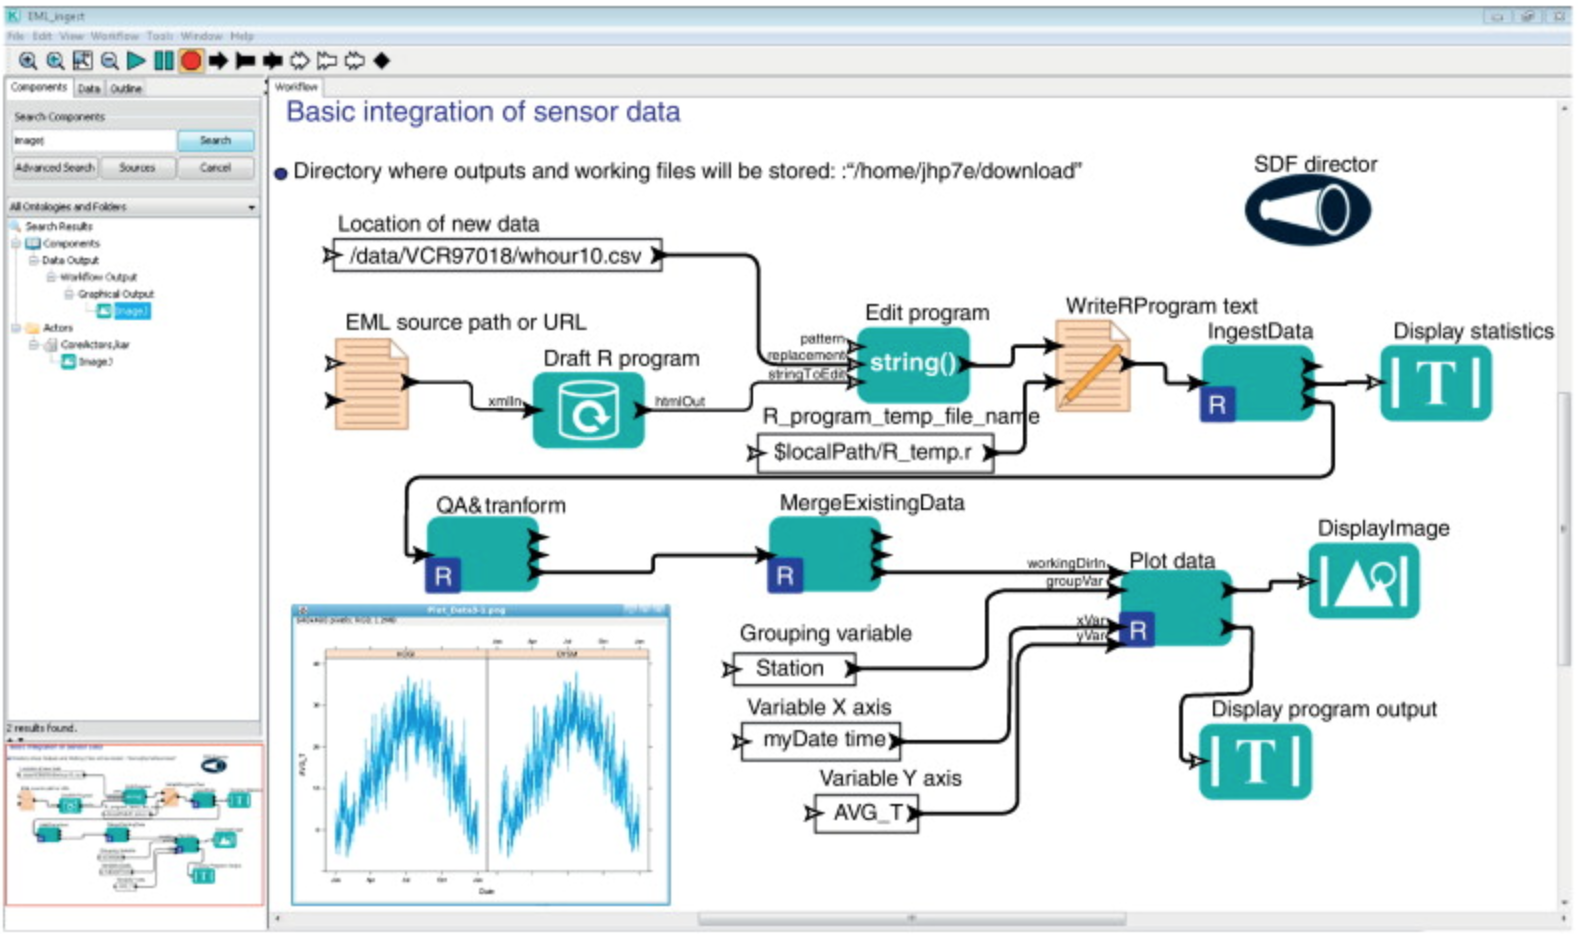
\includegraphics[scale=0.57]{tela_kepler.png}
	\caption{Interface gráfica do Kepler (retirado de \cite{kepler_screen}).}
	\label{fig:tela_kepler}
\end{figure}

Os \textit{workflows} gerados pelo sistema Kepler podem ser compartilhados a partir de uma representação XML (\textit{Extended Markup Language}) gerado pela própria linguagem de modelagem do \textit{Ptolemy} (\textit{MOML - Modeling Markup Language}). \\

\section{Vantagens na Utilização de um Sistema Gerenciador de \textit{Workflows} Científicos} \label{cap3sec5}

\textit{Workflows} científicos são projetados para ajudar os cientistas a realizar experimentos computacionais eficientes, proporcionando um ambiente que simplifica o desenho experimental, implementação e documentação. A crescente utilização de ambientes e sistemas de \textit{workflows} científicos é devido a uma série de vantagens que estes sistemas podem oferecer sobre abordagens alternativas, como:

\begin {itemize}
	\item \textit{Workflows} científicos automatizam tarefas repetitivas, permitindo que o usuário se concentre na ciência por trás do experimento, em vez de gastar tempo projetando o fluxo de dados e a gestão dos processos que compõem o \textit{workflow}. Por exemplo, a repetição de um mesmo experimento com o intuito de se calibrar parâmetros, processo este que pode ser repetido de à milhares de vezes, pode ser alcançado muito mais facilmente através da utilização de sistemas de \textit{workflows} do que com as abordagens convencionais de programação.	 
	\item \textit{Workflows} científicos documentam, explicitamente, o processo científico que está sendo executado, o que pode levar à uma melhor comunicação entre, por exemplo, uma equipe de cientistas ou uma comunidade acadêmica, colaboração (por exemplo, o compartilhamento de \textit{workflows} entre cientistas) e a reprodutibilidade dos resultados.
	\item Sistemas de \textit{workflows} científicos podem ser usado para monitorar a execução de \textit{workflows} e registrar a proveniência dos resultados de fluxo de trabalho. Proveniência, em particular, fornece uma forma de documentação que pode ser usado para validar e interpretar os resultados produzidos por (muitas vezes complexas) processos científicos.
	\item Sistemas de \textit{workflows} científico muitas vezes podem otimizar e executar de forma mais eficiente os processos científicos, por exemplo, ao expor e explorar várias formas de paralelismo inerente nos processos científicos orientados por dados, bem como pelo emprego de outras técnicas de gestão eficiente dos recursos.
	\item Ambientes de execução de \textit{workflows} incentivam a reutilização de artefatos de conhecimento (atores, fluxos de trabalho, conjuntos de dados, etc.) desenvolvidos ao se  automatizar um processo científico, tanto dentro como entre disciplinas.
\end {itemize}